\documentclass[aspectratio=169,xcolor=table]{beamer}

\usepackage{basileabeam}
\usepackage{hyperref}
\usepackage[english]{babel}
\usepackage[T1]{fontenc}
\usepackage{xcolor}
\usepackage{amssymb}
\usepackage{mathtools}
\usepackage{booktabs}
\usepackage{graphicx}
\usepackage{listings}
\usepackage{tikz}
\usetikzlibrary{arrows.meta,backgrounds,calc,fit,positioning,shapes.geometric}

\definecolor{unimint}{RGB}{30,165,165}
\definecolor{unilightmint}{RGB}{165,215,210}
\definecolor{unidark}{RGB}{45,55,60}
\definecolor{unigrey}{RGB}{140,145,150}
\definecolor{unired}{RGB}{210,5,55}
\definecolor{softblue}{RGB}{232,242,250}
\definecolor{softmint}{RGB}{232,247,245}
\definecolor{softred}{RGB}{252,235,239}
\definecolor{softgrey}{RGB}{244,245,246}

\setbeamerfont{footnote}{size=\tiny}
\setbeamerfont{caption}{size=\scriptsize}
\setbeamertemplate{caption}[numbered]
\setbeamercovered{invisible}

\newcommand{\code}[1]{\texttt{#1}}
\newcommand{\key}[1]{\textcolor{unired}{\textbf{#1}}}
\newcommand{\implemented}{\textcolor{unimint}{\textbf{Implemented}}}
\newcommand{\planned}{\textcolor{unired}{\textbf{Planned}}}

\tikzset{
  >={Latex[length=2.2mm]},
  flow/.style={-Latex, line width=0.75pt, draw=unidark},
  flowsoft/.style={-Latex, line width=0.65pt, draw=unigrey},
  box/.style={
    draw=unidark,
    rounded corners=1.5pt,
    fill=white,
    align=center,
    inner sep=4.5pt,
    font=\scriptsize
  },
  mintbox/.style={box, fill=softmint, draw=unimint},
  bluebox/.style={box, fill=softblue, draw=blue!55!black},
  redbox/.style={box, fill=softred, draw=unired},
  greybox/.style={box, fill=softgrey, draw=unigrey},
  groupbox/.style={
    draw=unigrey,
    rounded corners=2pt,
    fill=softgrey,
    inner sep=7pt
  },
  tinylabel/.style={font=\tiny, text=unigrey, align=center}
}

\lstset{
  basicstyle=\ttfamily\tiny,
  keywordstyle=\color{unired}\bfseries,
  commentstyle=\color{unigrey},
  stringstyle=\color{blue!60!black},
  showstringspaces=false,
  columns=fullflexible,
  keepspaces=true,
  frame=single,
  rulecolor=\color{unigrey},
  backgroundcolor=\color{softgrey},
  xleftmargin=0.25em,
  xrightmargin=0.25em,
  aboveskip=0.3em,
  belowskip=0.3em
}


\title{Interactive VR Museum for Image, Video and 3D Model Collections}
\author{Jannick Seper}
\email{\href{mailto:j.seper@stud.unibas.ch}{\textcolor{lcolor}{j.seper@stud.unibas.ch}}}
\institute{%
  Bachelor's Thesis --- Databases and Information Systems Group\\[1ex]
  Examiner: Prof. Dr. Heiko Schuldt\\
  Supervisors: Rahel Arnold and Raphael Waltenspül%
}

\date{08.09.2026}

\ulogo{Template/header}
\ulistelement{Template/listelement}
\graphicspath{{./images/}{../}}
\totalNoSlidesDisabled

\begin{document}

\input{content/01-title}
% 02-physical-exhibitions
\section{Motivation}
\begin{frame}[c]{Physical exhibitions}
\begin{columns}[T,onlytextwidth]
\begin{column}{0.30\textwidth}
\textcolor{unired}{\LARGE 01}

\vspace{0.15cm}
\large\textbf{Limited space}
\textcolor{unimint}{\rule{\linewidth}{1.6pt}}

\small Only part of a collection can be shown.
\end{column}
\begin{column}{0.30\textwidth}
\textcolor{unired}{\LARGE 02}

\vspace{0.15cm}
\large\textbf{Separate places}
\textcolor{unimint}{\rule{\linewidth}{1.6pt}}

\small Objects are spread across different institutions.
\end{column}
\begin{column}{0.30\textwidth}
\textcolor{unired}{\LARGE 03}

\vspace{0.15cm}
\large\textbf{Fragile originals}
\textcolor{unimint}{\rule{\linewidth}{1.6pt}}

\small Physical objects need care and protection.
\end{column}
\end{columns}
\end{frame}

% 03-digital-access
\begin{frame}[c]{Digital access}
\begin{columns}[c,onlytextwidth]
\begin{column}{0.43\textwidth}
\textcolor{unired}{\large\bfseries DIGITAL ACCESS}
\vspace{0.2cm}

Large collections, available anywhere.

\vspace{0.4cm}
\textcolor{unired}{\large\bfseries WHAT IS MISSING}
\vspace{0.2cm}

A shared space to explore the results.
\end{column}
\begin{column}{0.52\textwidth}
\centering
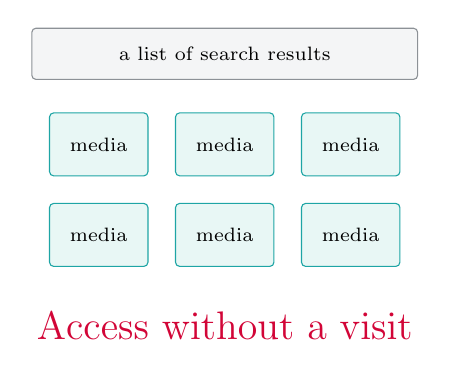
\begin{tikzpicture}
\node[greybox,minimum width=4.9cm,minimum height=0.65cm] at (0,1.8) {a list of search results};
\foreach \x in {-1.6,0,1.6}{
\foreach \y in {0.65,-0.5}{
\node[mintbox,minimum width=1.25cm,minimum height=0.8cm] at (\x,\y) {media};
}}
\node[font=\Large,text=unired] at (0,-1.65) {Access without a visit};
\end{tikzpicture}
\end{column}
\end{columns}
\end{frame}

% 04-research-question
\begin{frame}[c]{Research question}
\begin{beamercolorbox}[sep=1em,rounded=true]{palette highlight}
\centering\Large
How can a multimodal collection become a dynamic VR exhibition?
\end{beamercolorbox}
\vspace{0.6cm}
\centering\large
Text search to start. Similarity search to explore.

\vspace{0.3cm}
\normalsize Powered by vitrivr-engine.
\end{frame}

% 05-scope
\begin{frame}[c]{Scope}
\begin{columns}[T,onlytextwidth]
\begin{column}{0.47\textwidth}
\textcolor{unimint!80!black}{\large\bfseries IN SCOPE}
\textcolor{unimint}{\rule{\linewidth}{1.6pt}}
\begin{itemize}
\item Images, videos and 3D models
\item Text and similarity search
\item VR interaction and usability
\end{itemize}
\end{column}
\begin{column}{0.47\textwidth}
\textcolor{unired}{\large\bfseries OUT OF SCOPE}
\textcolor{unimint}{\rule{\linewidth}{1.6pt}}
\begin{itemize}
\item A new retrieval model
\item A finished application
\item A real museum reconstruction
\end{itemize}
\end{column}
\end{columns}
\end{frame}

% 06-system-overview
\section{Background}
\begin{frame}[c]{System overview}
\centering
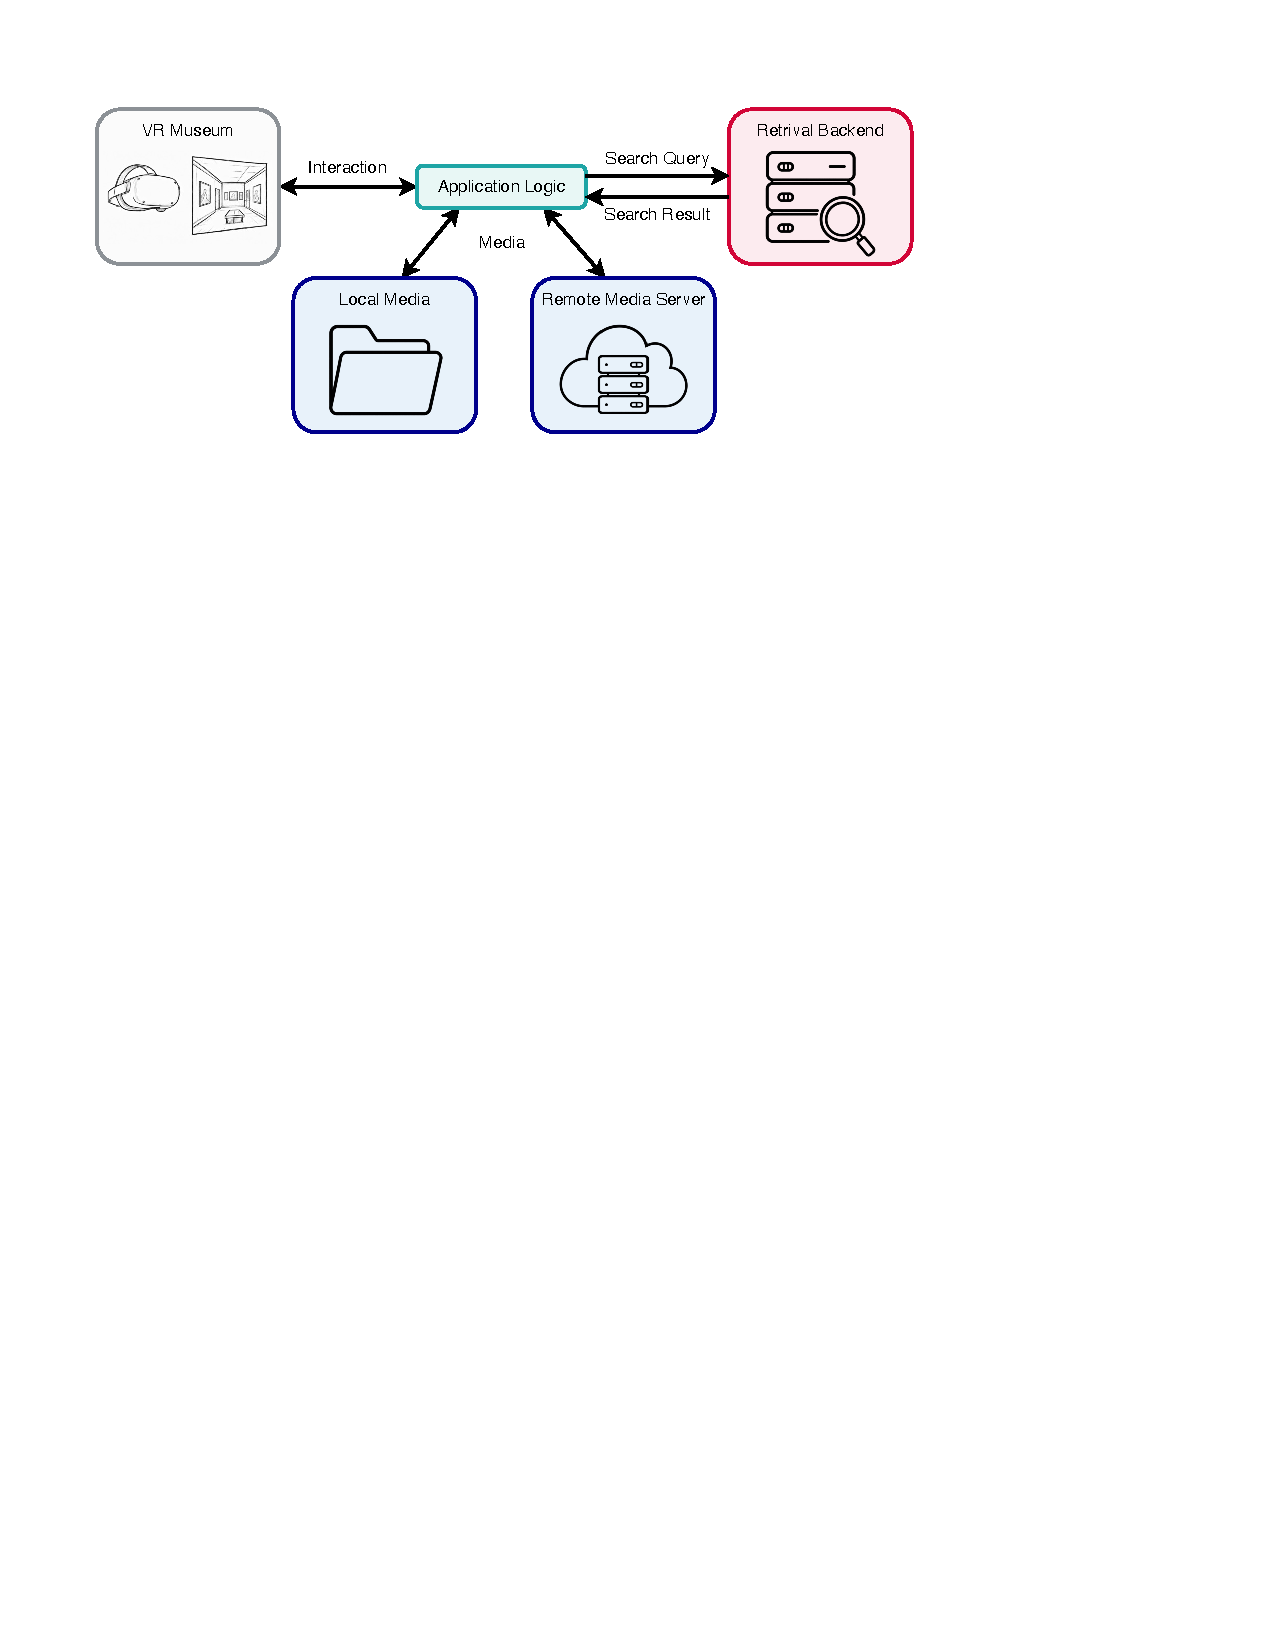
\includegraphics[width=0.87\linewidth,height=3.7cm,keepaspectratio]{Report/Figures/ch04-01-conceptual-architecture}

\vspace{0.25cm}
\begin{columns}[T,onlytextwidth]
\begin{column}{0.30\textwidth}
\centering\small\textbf{VR application}\\Godot \& OpenXR
\end{column}
\begin{column}{0.30\textwidth}
\centering\small\textbf{Search}\\vitrivr-engine
\end{column}
\begin{column}{0.30\textwidth}
\centering\small\textbf{Database}\\PostgreSQL with pgvector
\end{column}
\end{columns}
\end{frame}

% 07-xr
\begin{frame}[c]{XR}
\begin{columns}[T,onlytextwidth]
\begin{column}{0.30\textwidth}
\textcolor{unired}{\large\bfseries VR}

\small Virtual Reality
\textcolor{unimint}{\rule{\linewidth}{1.6pt}}

A fully virtual environment
\end{column}
\begin{column}{0.30\textwidth}
\textcolor{unired}{\large\bfseries AR}

\small Augmented Reality
\textcolor{unimint}{\rule{\linewidth}{1.6pt}}

Digital content over the real world
\end{column}
\begin{column}{0.30\textwidth}
\textcolor{unired}{\large\bfseries MR}

\small Mixed Reality
\textcolor{unimint}{\rule{\linewidth}{1.6pt}}

Digital objects integrated into real space
\end{column}
\end{columns}
\vspace{0.3cm}
\begin{columns}[c,onlytextwidth]
\begin{column}{0.36\textwidth}
\large This museum uses VR

\vspace{0.15cm}
\small Controllers or hand tracking
\end{column}
\begin{column}{0.28\textwidth}
\centering
\begin{tikzpicture}
  \node[inner sep=0,outer sep=0] (artwork) {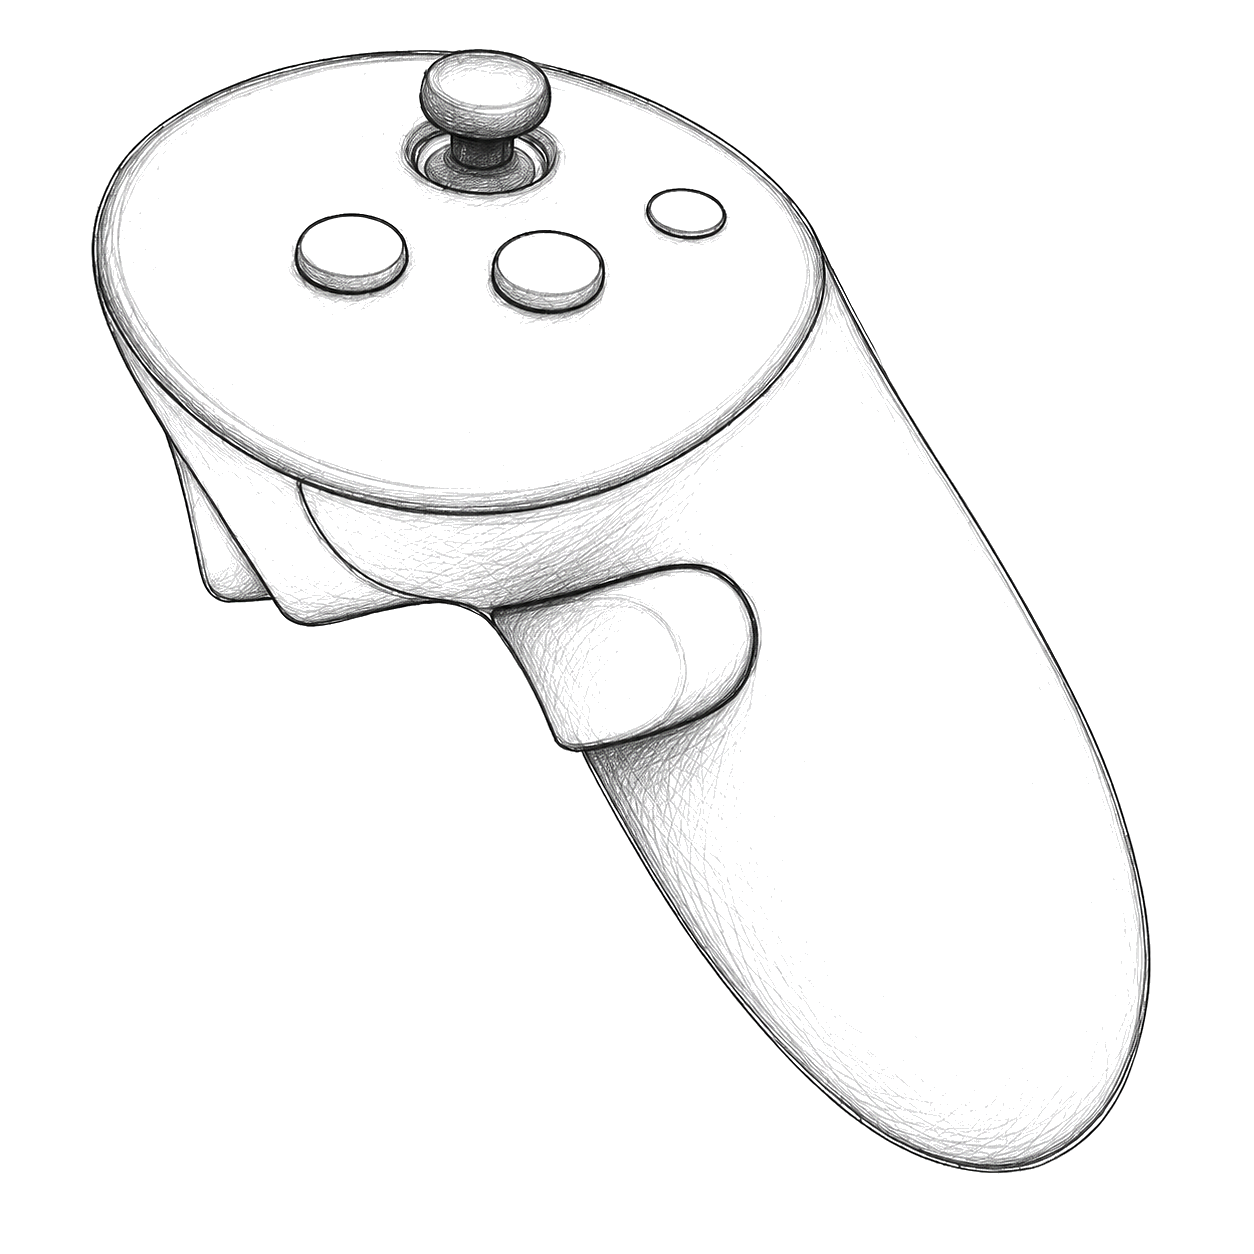
\includegraphics[height=2.05cm,width=\linewidth,keepaspectratio]{Report/Figures/ch04-02-interaction-controller.pdf}};
  \node[anchor=south east,inner sep=1pt,text=black!65,font=\fontsize{4}{5}\selectfont]
    at ([xshift=15pt,yshift=1pt]artwork.south east) {[GPT]};
\end{tikzpicture}

\small Controller
\end{column}
\begin{column}{0.28\textwidth}
\centering
\begin{tikzpicture}
  \node[inner sep=0,outer sep=0] (artwork) {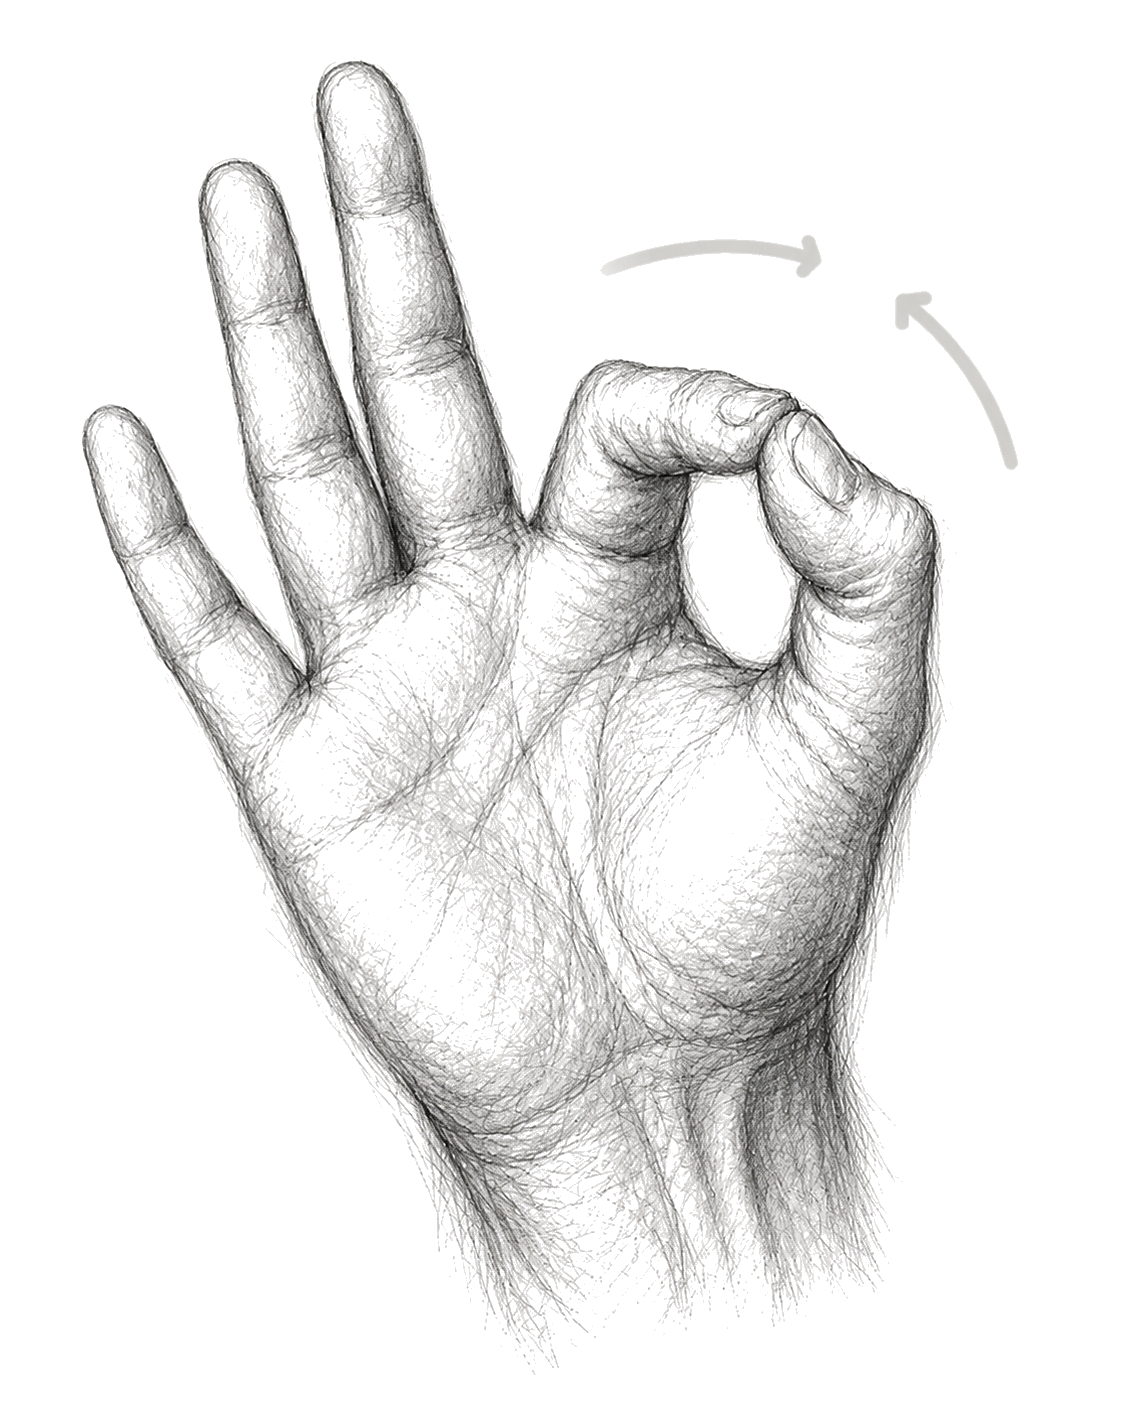
\includegraphics[height=2.05cm,width=\linewidth,keepaspectratio]{Report/Figures/ch04-02-interaction-pinch.pdf}};
  \node[anchor=south east,inner sep=1pt,text=black!65,font=\fontsize{4}{5}\selectfont]
    at ([xshift=15pt,yshift=1pt]artwork.south east) {[GPT]};
\end{tikzpicture}

\small Hand tracking
\end{column}
\end{columns}
\end{frame}

\input{content/08-clip}
% 09-3d-through-images
\begin{frame}[c]{3D through images}
\centering

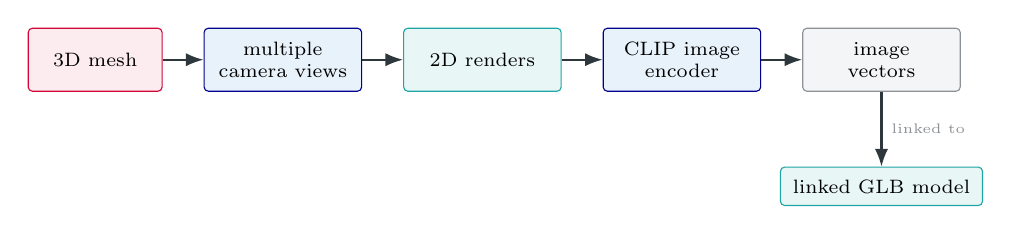
\begin{tikzpicture}[node distance=0.52cm, every node/.style={font=\scriptsize}]
  \node[redbox, minimum width=1.7cm, minimum height=0.8cm] (mesh) {3D mesh};
  \node[bluebox, right=of mesh, minimum width=2.0cm, minimum height=0.8cm] (views) {multiple\\camera views};
  \node[mintbox, right=of views, minimum width=2.0cm, minimum height=0.8cm] (renders) {2D renders};
  \node[bluebox, right=of renders, minimum width=2.0cm, minimum height=0.8cm] (clip) {CLIP image\\encoder};
  \node[greybox, right=of clip, minimum width=2.0cm, minimum height=0.8cm] (vectors) {image\\vectors};

  \draw[flow] (mesh) -- (views);
  \draw[flow] (views) -- (renders);
  \draw[flow] (renders) -- (clip);
  \draw[flow] (clip) -- (vectors);

  \node[mintbox, below=0.95cm of vectors, minimum width=2.0cm] (parent) {linked GLB model};
  \draw[flow] (vectors) -- node[right,tinylabel] {linked to} (parent);

\end{tikzpicture}

\vspace{0.65cm}
\begin{beamercolorbox}[sep=0.65em,rounded=true]{palette highlight}
\centering A matching view leads back to the original 3D model.
\end{beamercolorbox}
\end{frame}

% 10-three-media-pipelines
\begin{frame}[c]{Three media pipelines}
\centering
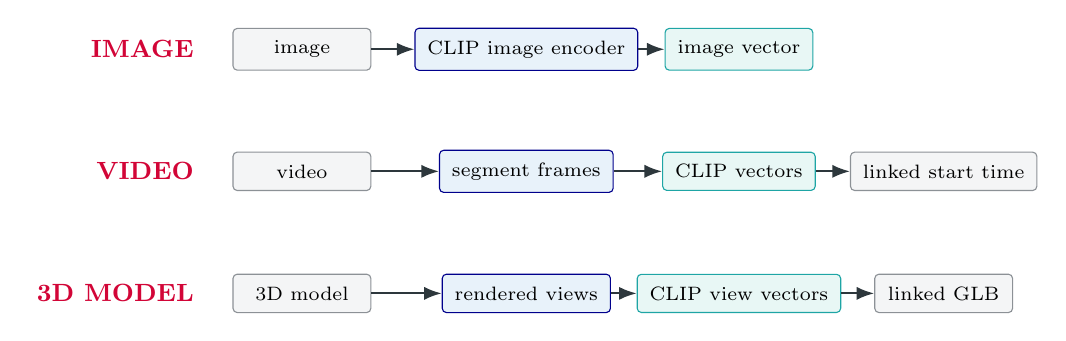
\begin{tikzpicture}[every node/.style={font=\scriptsize}]
  \node[anchor=east,font=\small\bfseries,text=unired] at (-4.55,1.55) {IMAGE};
  \node[greybox,minimum width=1.75cm] (image) at (-3.30,1.55) {image};
  \node[bluebox,minimum width=2.0cm] (imageclip) at (-0.45,1.55) {CLIP image encoder};
  \node[mintbox,minimum width=1.75cm] (imagevec) at (2.25,1.55) {image vector};
  \draw[flow] (image) -- (imageclip);
  \draw[flow] (imageclip) -- (imagevec);

  \node[anchor=east,font=\small\bfseries,text=unired] at (-4.55,0) {VIDEO};
  \node[greybox,minimum width=1.75cm] (video) at (-3.30,0) {video};
  \node[bluebox,minimum width=2.0cm] (frames) at (-0.45,0) {segment frames};
  \node[mintbox,minimum width=1.75cm] (videovec) at (2.25,0) {CLIP vectors};
  \node[greybox,minimum width=1.75cm] (time) at (4.85,0) {linked start time};
  \draw[flow] (video) -- (frames);
  \draw[flow] (frames) -- (videovec);
  \draw[flow] (videovec) -- (time);

  \node[anchor=east,font=\small\bfseries,text=unired] at (-4.55,-1.55) {3D MODEL};
  \node[greybox,minimum width=1.75cm] (model) at (-3.30,-1.55) {3D model};
  \node[bluebox,minimum width=2.0cm] (views) at (-0.45,-1.55) {rendered views};
  \node[mintbox,minimum width=1.75cm] (viewvec) at (2.25,-1.55) {CLIP view vectors};
  \node[greybox,minimum width=1.75cm] (glb) at (4.85,-1.55) {linked GLB};
  \draw[flow] (model) -- (views);
  \draw[flow] (views) -- (viewvec);
  \draw[flow] (viewvec) -- (glb);
\end{tikzpicture}

\vspace{0.30cm}
\small
Selected video frames and rendered 3D views share the same vector space as images.
\end{frame}

% 11-results-become-exhibits
\section{Concept}
\begin{frame}[c]{Results become exhibits}
\begin{columns}[c,onlytextwidth]
\begin{column}{0.36\textwidth}
\textcolor{unired}{\large\bfseries ONE ROOM}
\vspace{0.25cm}
\begin{itemize}
\item Images and videos on walls
\item 3D models on the floor
\item Selection and placement follow the ranking
\end{itemize}
\end{column}
\begin{column}{0.59\textwidth}
\centering
\begin{tikzpicture}
  \node[inner sep=0,outer sep=0] (artwork) {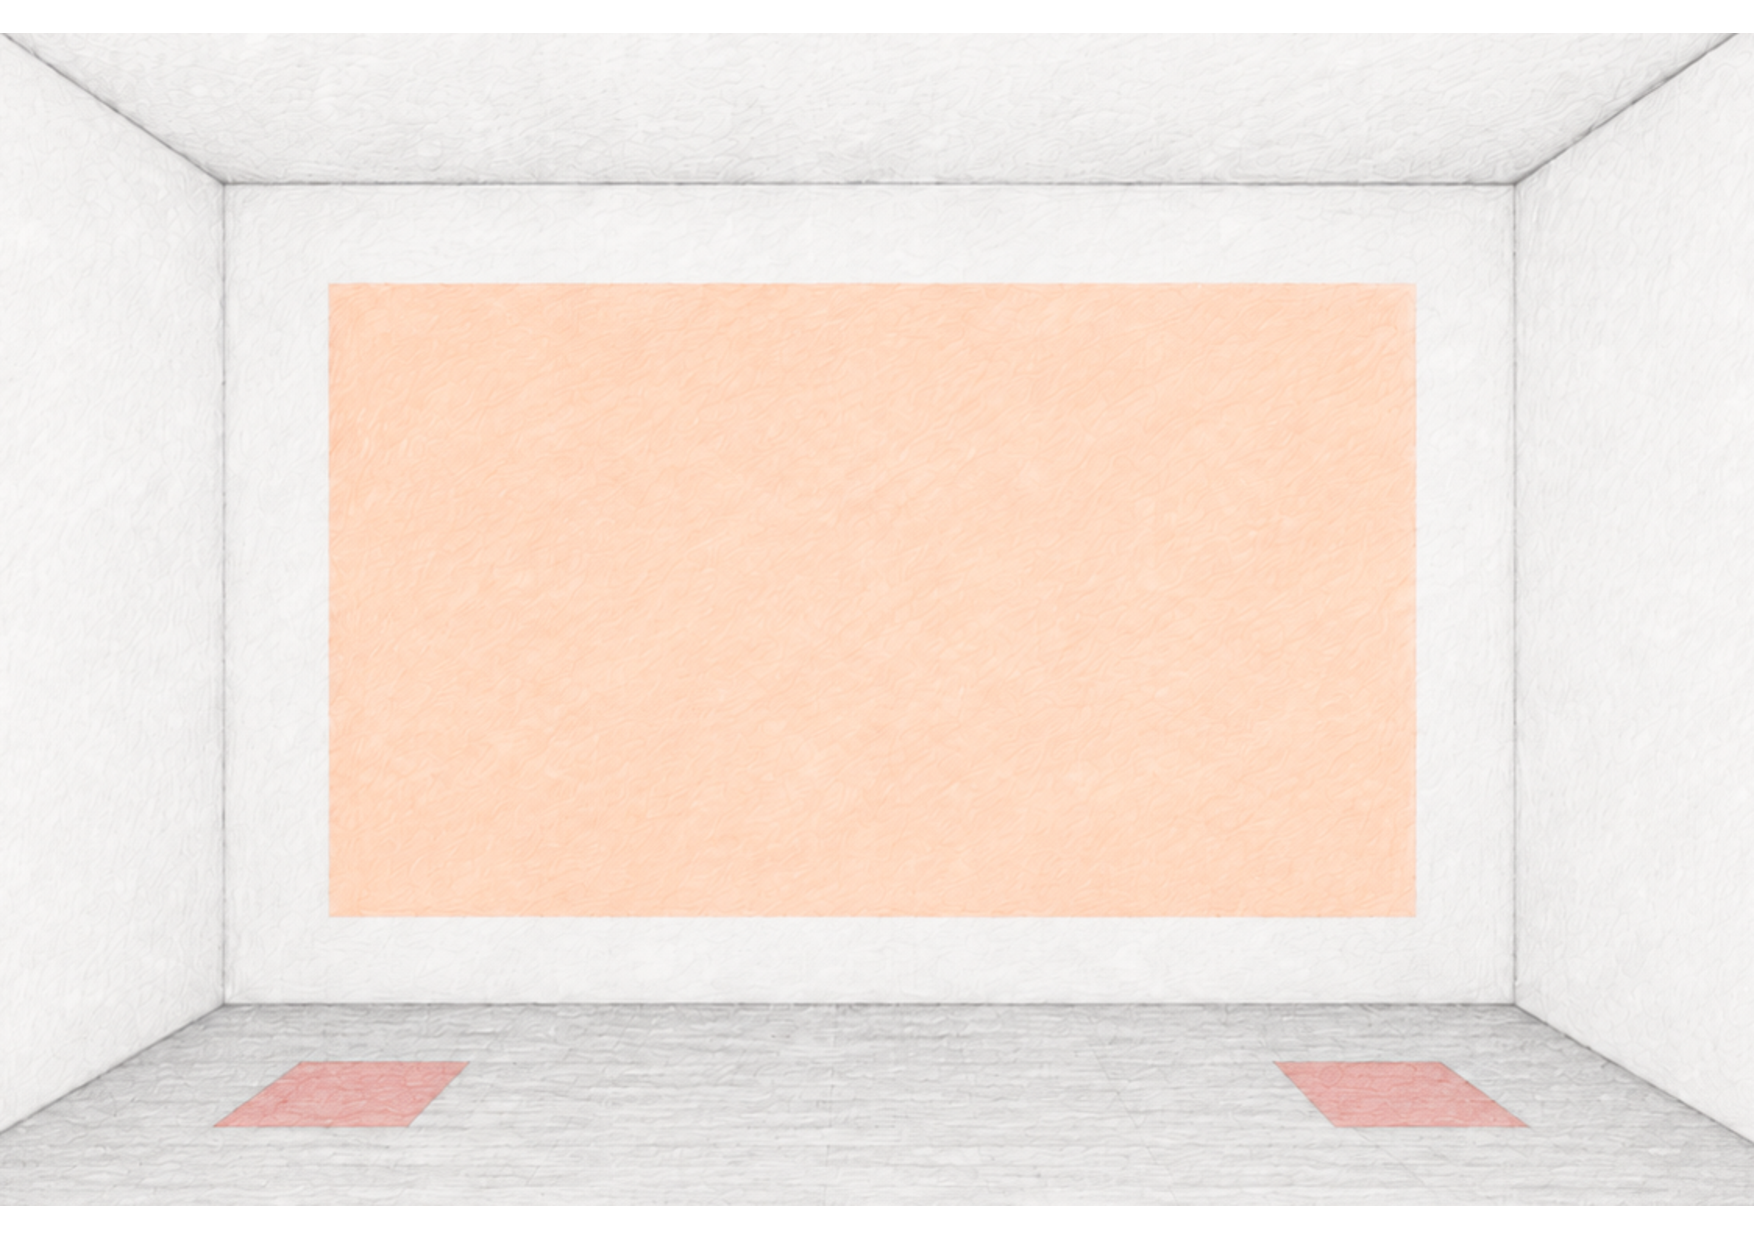
\includegraphics[width=\linewidth]{../Report/Figures/ch04-05-concept-placement-areas.pdf}};
  \node[anchor=south east,inner sep=1pt,text=black!65,font=\fontsize{4}{5}\selectfont]
    at ([yshift=5pt]artwork.south east) {[GPT]};
\end{tikzpicture}
\end{column}
\end{columns}
\end{frame}

% 12-two-exhibit-types
\begin{frame}[c]{Two exhibit types}
\begin{columns}[T,onlytextwidth]
  \begin{column}{0.48\textwidth}
    \centering
    \begin{tikzpicture}
      \node[inner sep=0,outer sep=0] (artwork) {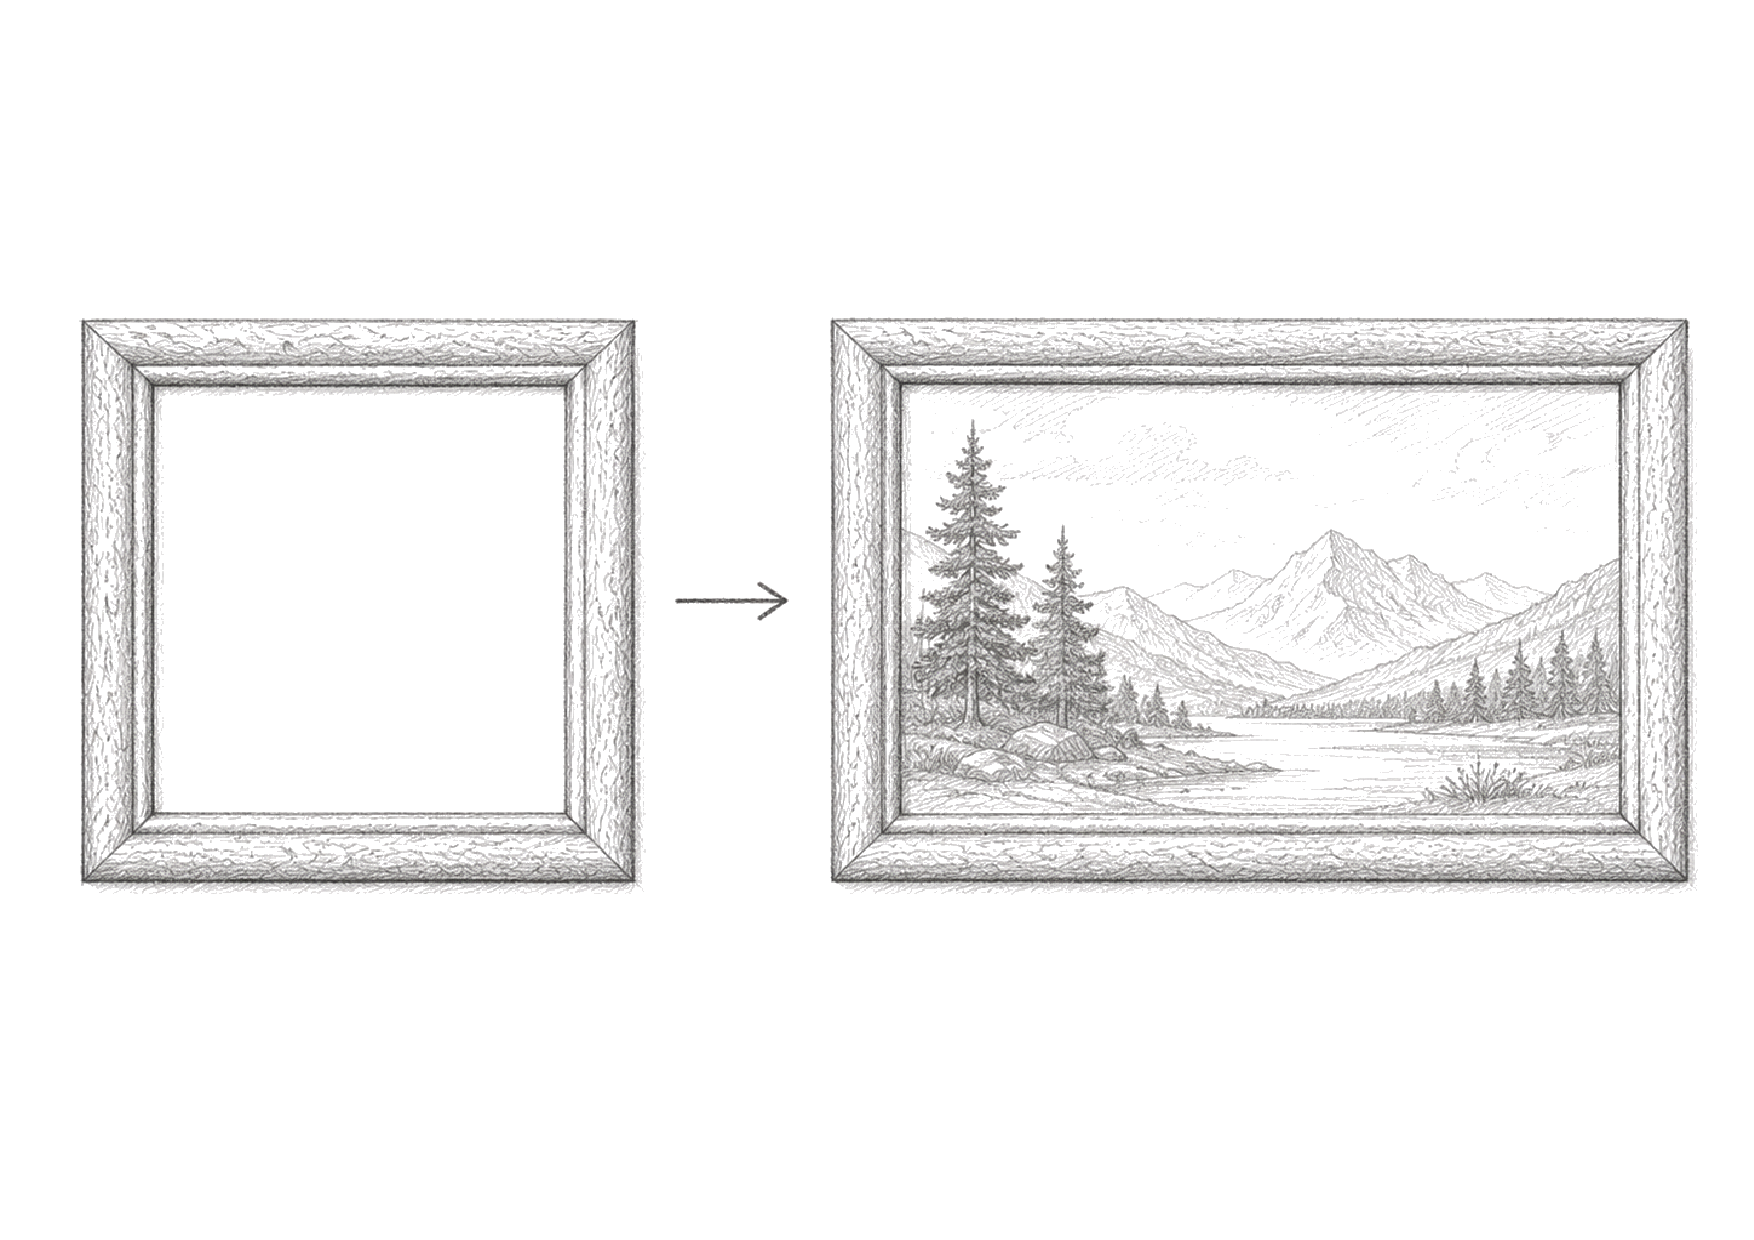
\includegraphics[height=3.35cm,keepaspectratio]{../Report/Figures/ch04-03-concept-2d-frame.pdf}};
      \node[anchor=south east,inner sep=1pt,text=black!65,font=\fontsize{4}{5}\selectfont]
        at ([xshift=-1pt,yshift=1pt]artwork.south east) {[GPT]};
    \end{tikzpicture}

    \vspace{0.10cm}
    \textcolor{unired}{\large\bfseries IMAGES \& VIDEOS}

    \vspace{0.08cm}
    \small
    Frames adapt to the media. Videos start at the matching segment.
  \end{column}
  \begin{column}{0.48\textwidth}
    \centering
    \begin{tikzpicture}
      \node[inner sep=0,outer sep=0] (artwork) {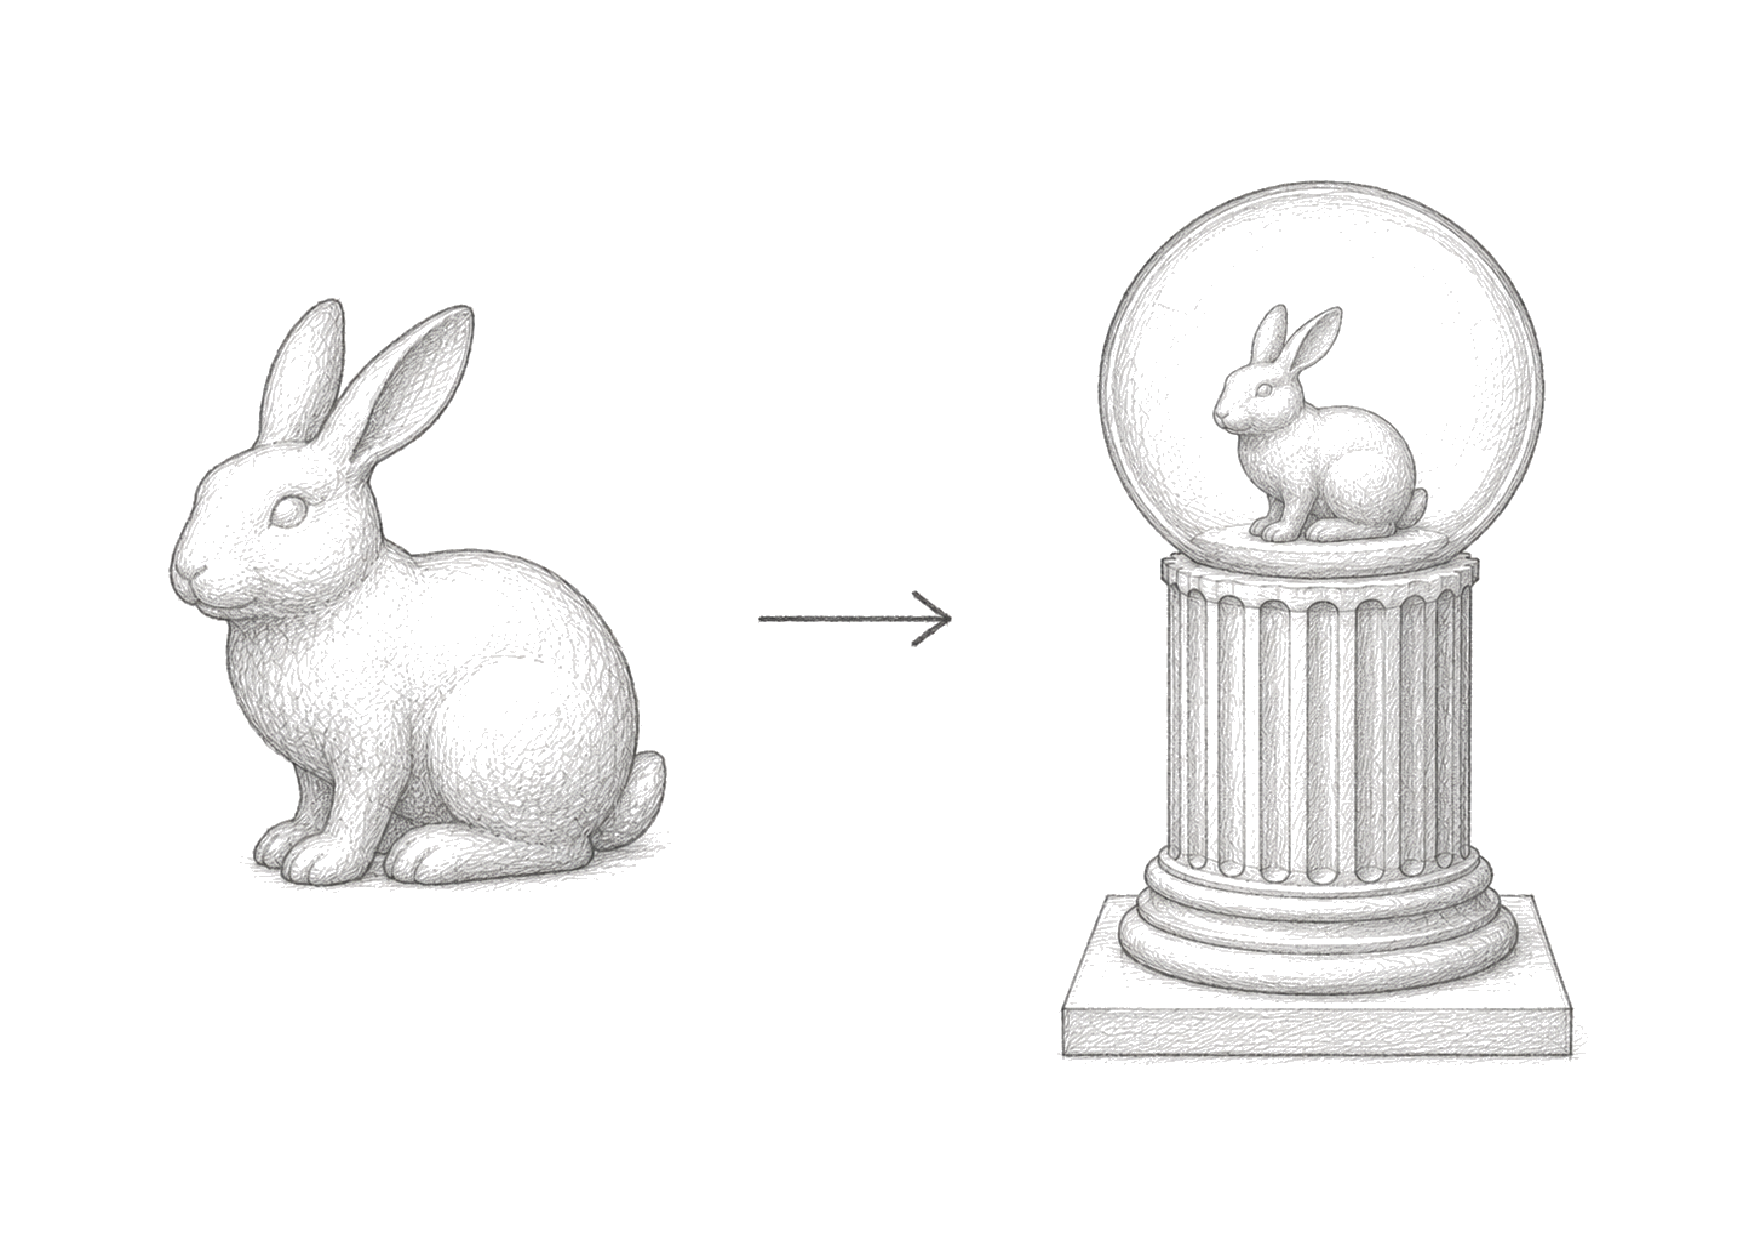
\includegraphics[height=3.35cm,keepaspectratio]{../Report/Figures/ch04-04-concept-3d-display.pdf}};
      \node[anchor=south east,inner sep=1pt,text=black!65,font=\fontsize{4}{5}\selectfont]
        at ([xshift=-1pt,yshift=1pt]artwork.south east) {[GPT]};
    \end{tikzpicture}

    \vspace{0.10cm}
    \textcolor{unired}{\large\bfseries 3D MODELS}

    \vspace{0.08cm}
    \small
    A fitted display. Inspection from every side.
  \end{column}
\end{columns}
\end{frame}

% 13-why-limit-results
\begin{frame}[c]{Why limit results?}
\begin{columns}[c,onlytextwidth]
  \begin{column}{0.50\textwidth}
    \centering
    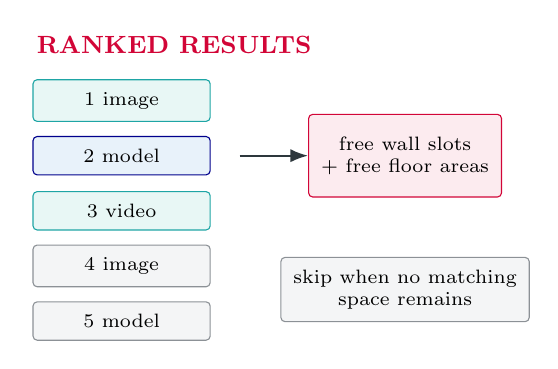
\begin{tikzpicture}[every node/.style={font=\scriptsize}]
      \node[anchor=west,font=\small\bfseries,text=unired] at (-2.65,1.75) {RANKED RESULTS};
      \foreach \y/\label/\style in {1.05/{1 image}/mintbox,0.35/{2 model}/bluebox,-0.35/{3 video}/mintbox,-1.05/{4 image}/greybox,-1.75/{5 model}/greybox}{
        \node[\style,minimum width=2.25cm,minimum height=0.48cm] at (-1.45,\y) {\label};
      }
      \node[redbox,minimum width=2.45cm,minimum height=1.05cm] (capacity) at (2.15,0.35) {free wall slots\\+ free floor areas};
      \draw[flow] (0.05,0.35) -- (capacity.west);
      \node[greybox,minimum width=2.45cm,minimum height=0.70cm] at (2.15,-1.35) {skip when no matching\\space remains};
    \end{tikzpicture}
  \end{column}
  \begin{column}{0.46\textwidth}
    \textcolor{unimint!80!black}{\large\bfseries WHY THIS MATTERS}

    \vspace{0.12cm}
    \small
    \begin{itemize}
      \item Keep the exhibition walkable.
      \item Respect wall and floor capacity.
      \item Select in retrieval order.
      \item Avoid unnecessary loading and resource use.
    \end{itemize}
  \end{column}
\end{columns}
\end{frame}

% 14-keep-exploring
\begin{frame}[c]{Keep exploring}
\centering
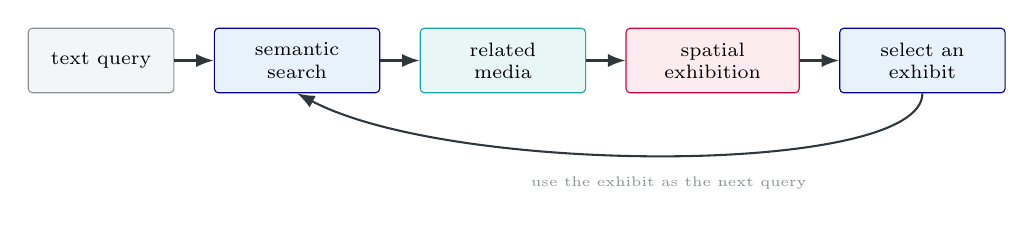
\begin{tikzpicture}[node distance=0.50cm,every node/.style={font=\scriptsize}]
  \node[greybox,minimum width=1.85cm,minimum height=0.82cm]
    (query) {text query};
  \node[bluebox,right=of query,minimum width=2.10cm,minimum height=0.82cm]
    (search) {semantic\\search};
  \node[mintbox,right=of search,minimum width=2.10cm,minimum height=0.82cm]
    (results) {related\\media};
  \node[redbox,right=of results,minimum width=2.20cm,minimum height=0.82cm]
    (exhibition) {spatial\\exhibition};
  \node[bluebox,right=of exhibition,minimum width=2.10cm,minimum height=0.82cm]
    (select) {select an\\exhibit};

  \foreach \a/\b in {query/search,search/results,results/exhibition,exhibition/select}
    \draw[flow] (\a) -- (\b);

  \draw[flow]
    (select.south) .. controls +(0,-1.05) and +(2.0,-1.05) ..
    node[below=4pt,tinylabel] {use the exhibit as the next query}
    (search.south);
\end{tikzpicture}

\vspace{0.45cm}
\begin{columns}[T,onlytextwidth]
  \begin{column}{0.44\textwidth}
    \centering
    \textcolor{unimint!80!black}{\large\bfseries FIRST ENTRY}

    \vspace{0.08cm}
    \small Start with a text query.
  \end{column}
  \begin{column}{0.44\textwidth}
    \centering
    \textcolor{unimint!80!black}{\large\bfseries CONTINUATION}

    \vspace{0.08cm}
    \small Select an exhibit and choose \emph{Similar}.
  \end{column}
\end{columns}
\end{frame}

% 15-separation-in-code
\section{Implementation}
\begin{frame}[c]{Separation in code}
\centering
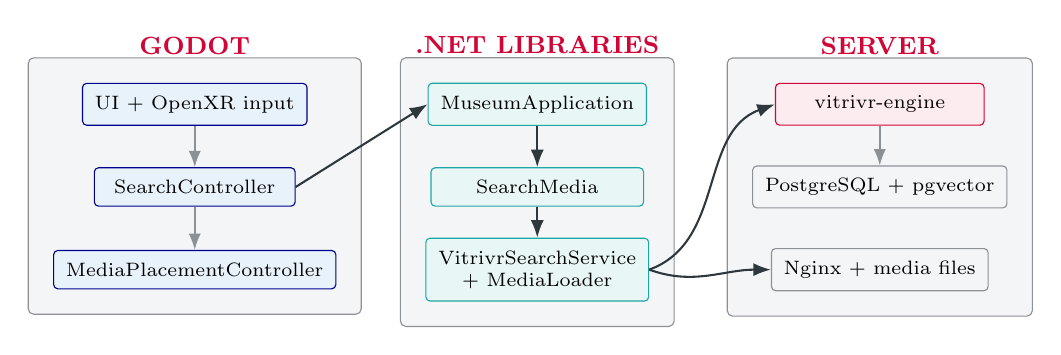
\begin{tikzpicture}[every node/.style={font=\scriptsize}]
  % Godot
  \node[bluebox,minimum width=2.55cm] (ui) at (-4.35,1.05) {UI + OpenXR input};
  \node[bluebox,minimum width=2.55cm] (controller) at (-4.35,0.00) {SearchController};
  \node[bluebox,minimum width=2.55cm] (placement) at (-4.35,-1.05) {MediaPlacementController};

  % Application libraries
  \node[mintbox,minimum width=2.70cm] (app) at (0,1.05) {MuseumApplication};
  \node[mintbox,minimum width=2.70cm] (search) at (0,0.00) {SearchMedia};
  \node[mintbox,minimum width=2.70cm] (adapters) at (0,-1.05) {VitrivrSearchService\\+ MediaLoader};

  % Server
  \node[redbox,minimum width=2.65cm] (engine) at (4.35,1.05) {vitrivr-engine};
  \node[greybox,minimum width=2.65cm] (database) at (4.35,0.00) {PostgreSQL + pgvector};
  \node[greybox,minimum width=2.65cm] (media) at (4.35,-1.05) {Nginx + media files};

  % Runtime path
  \draw[flowsoft] (ui) -- (controller);
  \draw[flowsoft] (controller) -- (placement);
  \draw[flow] (controller.east) -- (app.west);
  \draw[flow] (app) -- (search);
  \draw[flow] (search) -- (adapters);
  \draw[flow] (adapters.east) to[out=20,in=200] (engine.west);
  \draw[flowsoft] (engine) -- (database);
  \draw[flow] (adapters.east) to[out=-20,in=180] (media.west);

  \begin{scope}[on background layer]
    \node[groupbox,fit=(ui)(controller)(placement),inner sep=9pt] {};
    \node[groupbox,fit=(app)(search)(adapters),inner sep=9pt] {};
    \node[groupbox,fit=(engine)(database)(media),inner sep=9pt] {};
  \end{scope}

  \node[font=\small\bfseries,text=unired,above=0.24cm of ui] {GODOT};
  \node[font=\small\bfseries,text=unired,above=0.24cm of app] {.NET LIBRARIES};
  \node[font=\small\bfseries,text=unired,above=0.24cm of engine] {SERVER};
\end{tikzpicture}

\vspace{0.38cm}
\small
Search and loading stay separate from scenes. Media are loaded locally first and from Nginx if missing.
\end{frame}

% 16-exhibit-implementation
\begin{frame}[c]{Exhibit implementation}
\begin{columns}[T,onlytextwidth]
  \begin{column}{0.48\textwidth}
    \centering
    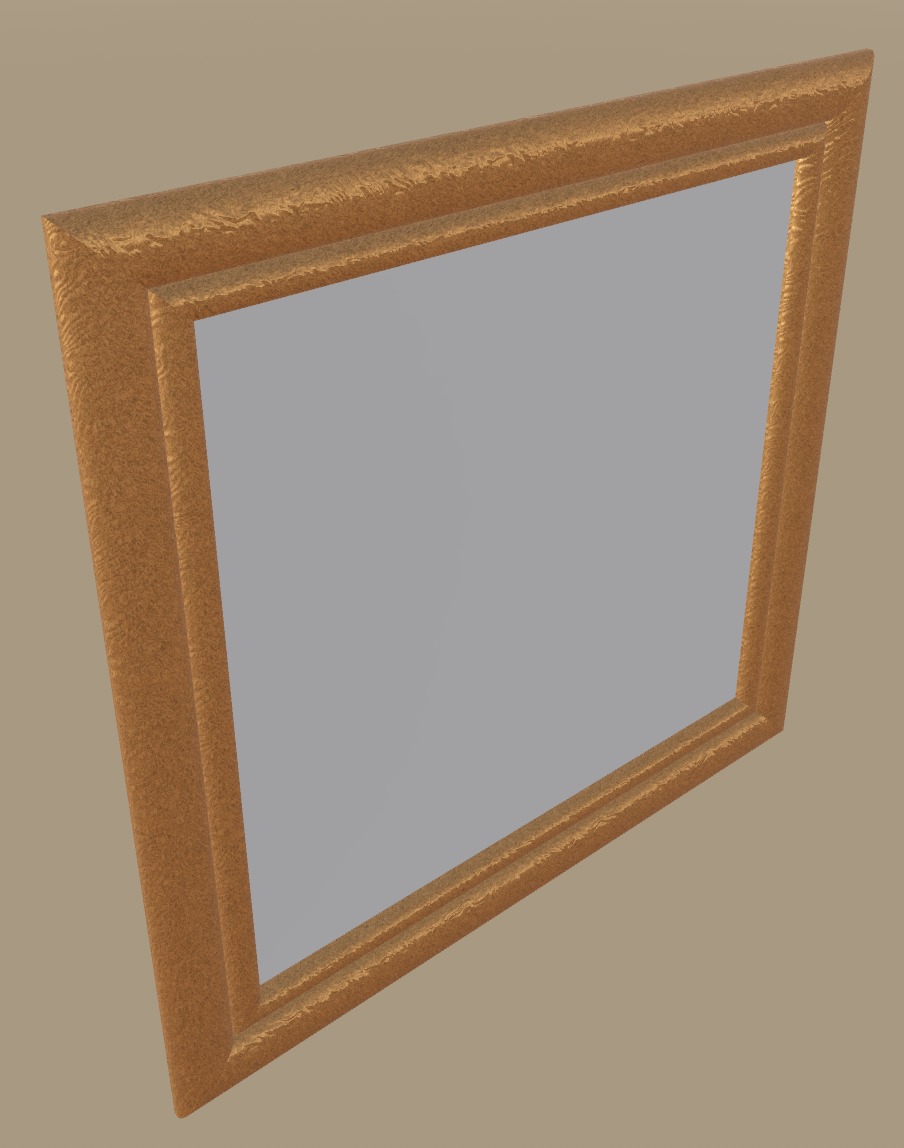
\includegraphics[height=3.12cm,keepaspectratio]{../Report/Figures/ch04-04-2d-frame.png}

    \vspace{0.08cm}
    \textcolor{unired}{\large\bfseries 2D EXHIBIT}

    \vspace{0.07cm}
    \footnotesize
    Adaptive frame and video playback.
  \end{column}
  \begin{column}{0.48\textwidth}
    \centering
    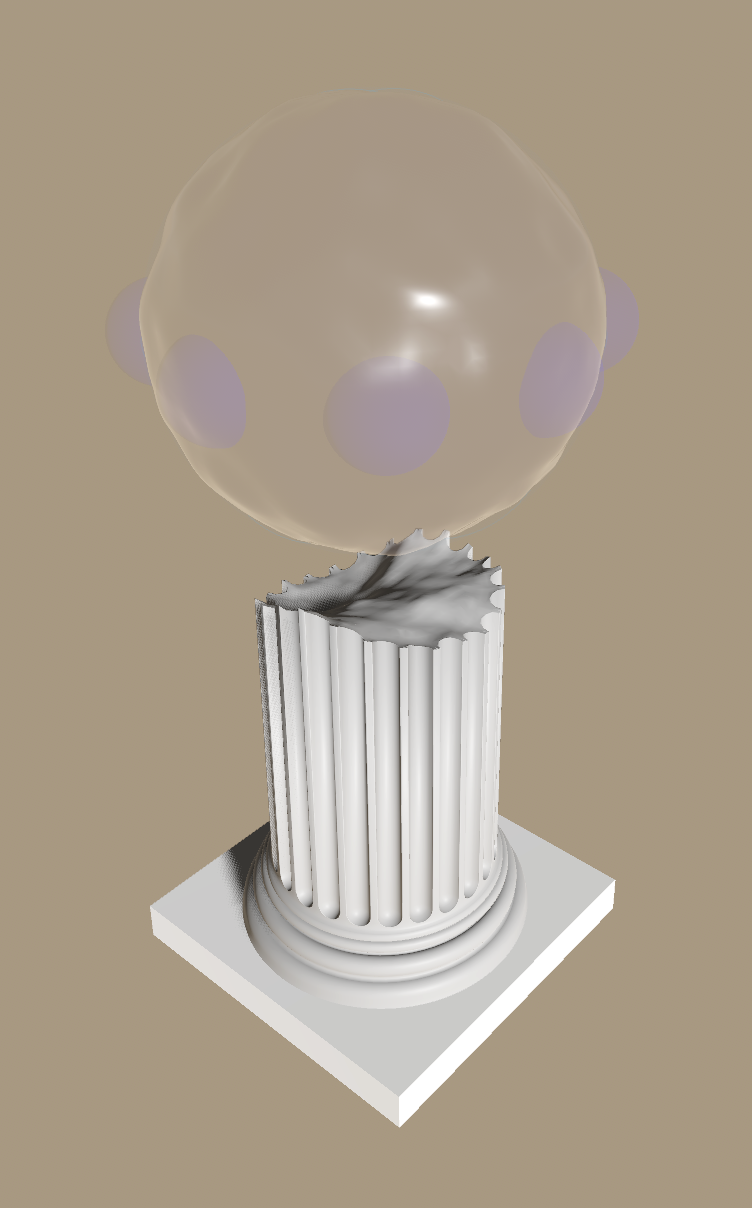
\includegraphics[height=3.12cm,keepaspectratio]{../Report/Figures/ch04-05-3d-orb-pillar.png}

    \vspace{0.08cm}
    \textcolor{unired}{\large\bfseries 3D EXHIBIT}

    \vspace{0.07cm}
    \footnotesize
    Fit, rotate and inspect in a separate room.
  \end{column}
\end{columns}

\vspace{0.18cm}
\begin{beamercolorbox}[sep=0.48em,rounded=true]{palette highlight}
  \centering\small
  Each exhibit carries the vector for \emph{Similar}.
\end{beamercolorbox}
\end{frame}

% 17-three-deployments
\begin{frame}[c]{Three deployments}
\begin{columns}[T,onlytextwidth]
  \begin{column}{0.30\textwidth}
    \textcolor{unired}{\LARGE 01}

    \vspace{0.08cm}
    \large\textbf{Quest 3}

    \vspace{0.12cm}
    \color{unimint}\rule{\linewidth}{1.6pt}
    \color{black}

    \vspace{0.18cm}
    \small
    Android standalone.\\
Controllers + hands.
  \end{column}
  \begin{column}{0.30\textwidth}
    \textcolor{unired}{\LARGE 02}

    \vspace{0.08cm}
    \large\textbf{VIVE Focus 3}

    \vspace{0.12cm}
    \color{unimint}\rule{\linewidth}{1.6pt}
    \color{black}

    \vspace{0.18cm}
    \small
    Android standalone.\\
Controllers + hands.
  \end{column}
  \begin{column}{0.30\textwidth}
    \textcolor{unired}{\LARGE 03}

    \vspace{0.08cm}
    \large\textbf{Windows stream}

    \vspace{0.12cm}
    \color{unimint}\rule{\linewidth}{1.6pt}
    \color{black}

    \vspace{0.18cm}
    \small
    Windows build streamed to a VR headset.
  \end{column}
\end{columns}

\vspace{0.52cm}
\begin{beamercolorbox}[sep=0.56em,rounded=true]{palette highlight}
  \centering\small
  One museum workflow, shared through OpenXR.
\end{beamercolorbox}
\end{frame}

% 18-demo
\section{Demo}
\begin{frame}[c,plain]
\centering
\Huge Demo

\vspace{0.65cm}
\large
Text search $\rightarrow$ exhibition $\rightarrow$ similarity search $\rightarrow$ model view

\end{frame}

% 19-user-study
\section{Evaluation}
\begin{frame}[c]{User study}
\begin{columns}[T,onlytextwidth]
\begin{column}{0.30\textwidth}
\textcolor{unired}{\LARGE\textbf{9}}
\textcolor{unimint}{\rule{\linewidth}{1.6pt}}
\large Participants

\vspace{0.2cm}
\small 22 device sessions:\\Quest: 8, Focus: 7,\newline Stream: 7
\end{column}
\begin{column}{0.30\textwidth}
\textcolor{unired}{\LARGE\textbf{3}}
\textcolor{unimint}{\rule{\linewidth}{1.6pt}}
\large Test setups

\vspace{0.2cm}
\small Search, explore,\\rotate, view at original size
\end{column}
\begin{column}{0.30\textwidth}
\textcolor{unired}{\LARGE\textbf{2}}
\textcolor{unimint}{\rule{\linewidth}{1.6pt}}
\large Types of feedback

\vspace{0.2cm}
\small Overall SUS\\Ratings and comments
\end{column}
\end{columns}
\end{frame}

% 20-overall-success
\begin{frame}[c]{Overall success}
\centering
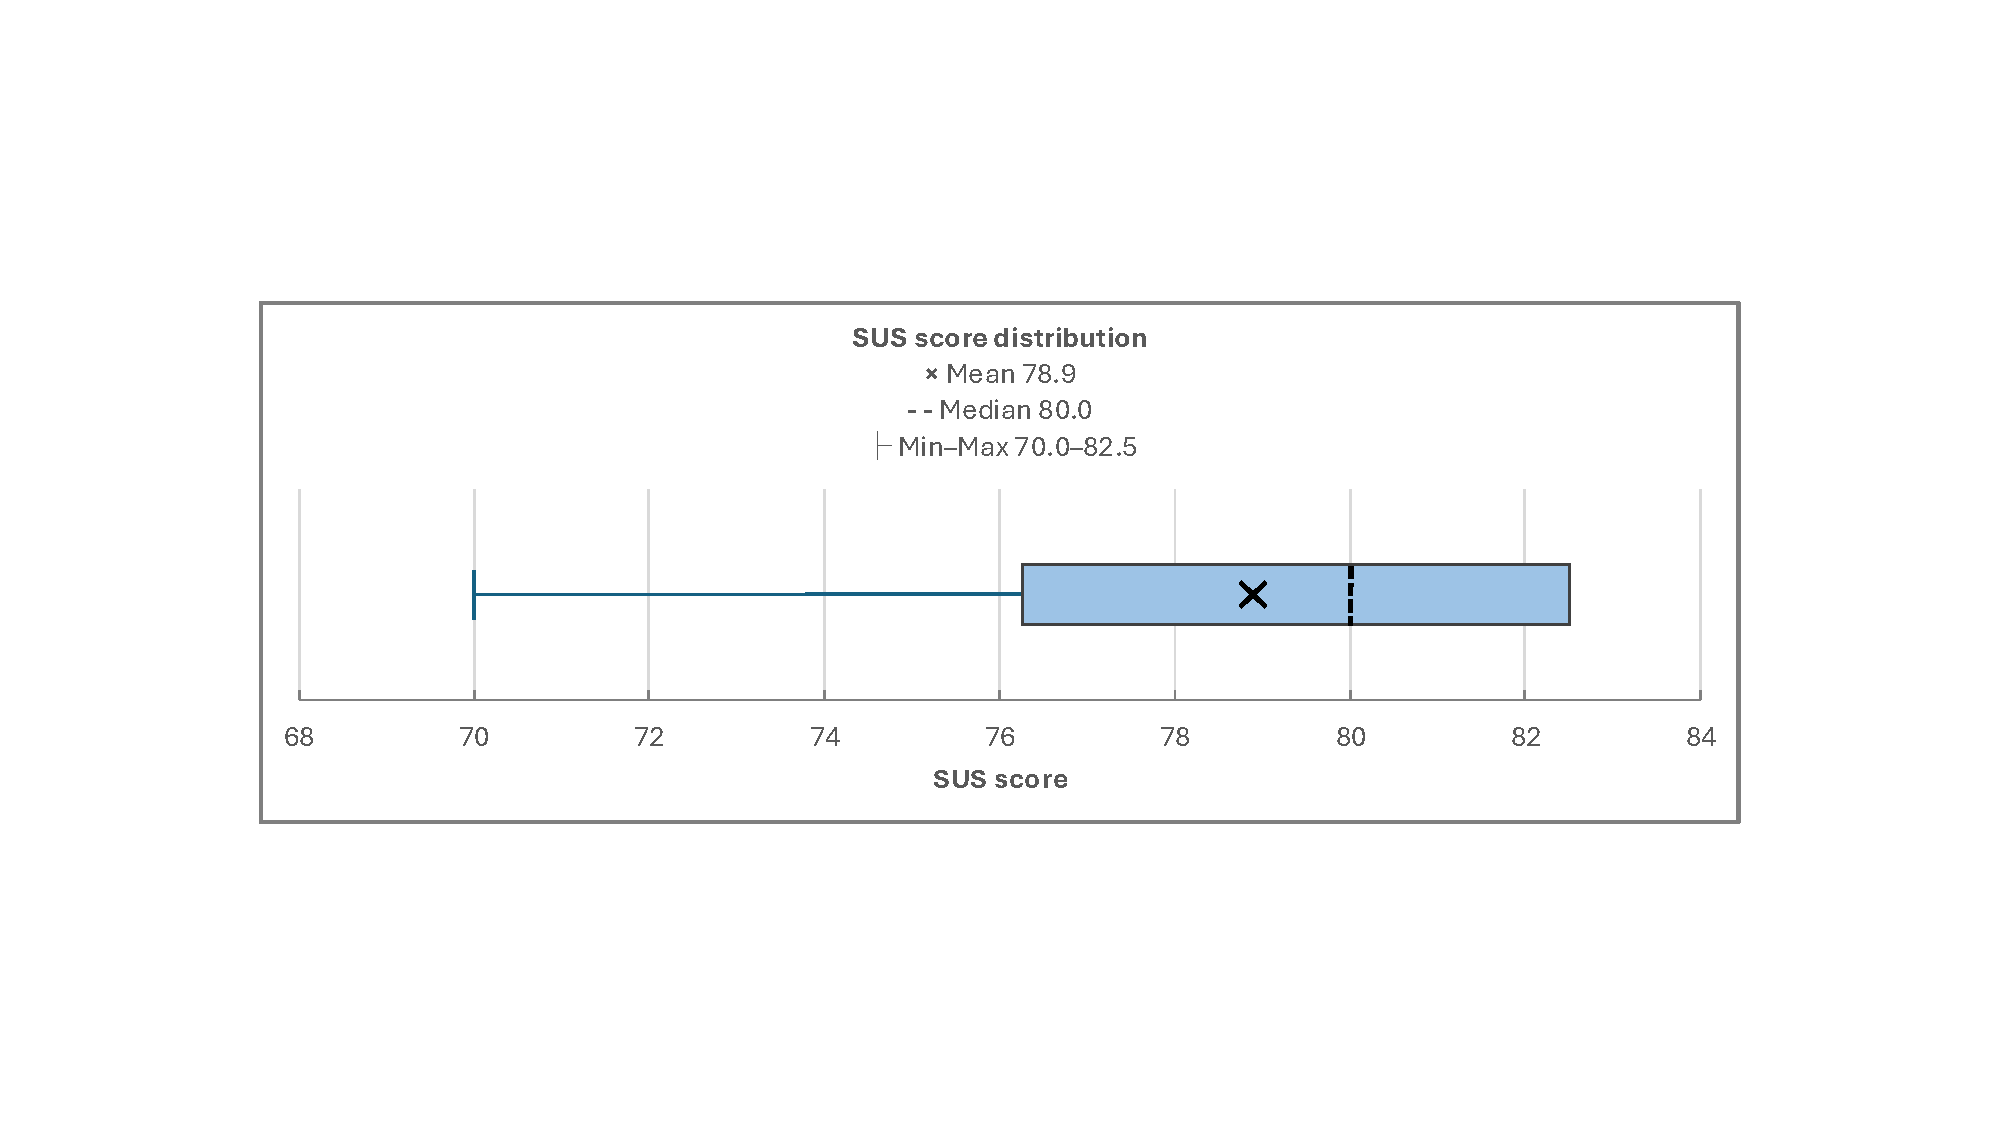
\includegraphics[width=0.87\linewidth]{../Report/Figures/ch06-01-sus-score-distribution.pdf}

\vspace{0.20cm}
\begin{columns}[c,onlytextwidth]
  \begin{column}{0.31\textwidth}
    \centering
    \textcolor{unired}{\LARGE\textbf{78.9}}\\[-0.03cm]
    \small mean
  \end{column}
  \begin{column}{0.31\textwidth}
    \centering
    \textcolor{unired}{\LARGE\textbf{80.0}}\\[-0.03cm]
    \small median
  \end{column}
  \begin{column}{0.31\textwidth}
    \centering
    \textcolor{unired}{\LARGE\textbf{70 to 82.5}}\\[-0.03cm]
    \small observed range
  \end{column}
\end{columns}
\vspace{0.40cm}
The box represents the range containing the middle 50\% of all SUS scores out of 100.
\end{frame}

% 21-what-worked-and-what-varied
\begin{frame}[c]{What worked and what varied}
\begin{columns}[c,onlytextwidth]
\begin{column}{0.35\textwidth}
\textcolor{unired}{\LARGE\textbf{22/22}}\\
Original-size viewing\\

\vspace{0.4cm}
\textcolor{unired}{\large\textbf{8/9}} layout \qquad
\textcolor{unired}{\large\textbf{9/9}} lighting
\end{column}
\begin{column}{0.60\textwidth}
\centering
\small Positive ratings
\vspace{0.15cm}

\begin{tabular}{lccc}
\toprule
& Quest & Focus & Stream\\
\midrule
Response speed & 5/8 & 3/7 & 7/7\\
Rotation & 6/8 & 4/7 & 6/7\\
Controllers & 6/8 & 3/7 & 6/7\\
Hands & 6/8 & 3/7 & --\\
\bottomrule
\end{tabular}
\end{column}
\end{columns}
\vspace{0.5cm}
\begin{beamercolorbox}[sep=0.55em,rounded=true]{palette highlight}
\centering\small Different file loading conditions mean this is not a hardware comparison.
\end{beamercolorbox}
\end{frame}

% 22-what-still-needs-work
\begin{frame}[c]{What still needs work}
\begin{columns}[T,onlytextwidth]
\begin{column}{0.30\textwidth}
\textcolor{unired}{\large\bfseries GUIDANCE}
\textcolor{unimint}{\rule{\linewidth}{1.6pt}}

Instructions are hard to remember.

\vspace{0.25cm}
\small Reopen the tutorial.\\Label buttons and gestures.
\end{column}
\begin{column}{0.30\textwidth}
\textcolor{unired}{\large\bfseries FEEDBACK}
\textcolor{unimint}{\rule{\linewidth}{1.6pt}}

Changes need clearer signals.

\vspace{0.25cm}
\small Clearer signals for loading\\and exhibition changes.
\end{column}
\begin{column}{0.30\textwidth}
\textcolor{unired}{\large\bfseries INTERACTION}
\textcolor{unimint}{\rule{\linewidth}{1.6pt}}

Rotation needs refinement.

\vspace{0.25cm}
\small Simpler controls.\\Lower default speeds.
\end{column}
\end{columns}
\vspace{0.5cm}
\begin{beamercolorbox}[sep=0.55em,rounded=true]{palette highlight}
\centering\small Further requests include search history and metadata.
\end{beamercolorbox}
\end{frame}

% 23-search-becomes-a-visit
\section{Conclusion}
\begin{frame}[c]{Search becomes a visit}
\begin{beamercolorbox}[sep=0.9em,rounded=true]{palette highlight}
\centering\Large One room. Three media types. New paths through Similar.
\end{beamercolorbox}
\vspace{0.55cm}
\begin{columns}[T,onlytextwidth]
\begin{column}{0.30\textwidth}
\textcolor{unired}{\large\bfseries BUILT}

\vspace{0.15cm}
A working multimodal VR museum.
\end{column}
\begin{column}{0.30\textwidth}
\textcolor{unired}{\large\bfseries TESTED}

\vspace{0.15cm}
Usable for the study group.
\end{column}
\begin{column}{0.30\textwidth}
\textcolor{unired}{\large\bfseries NEXT}

\vspace{0.15cm}
Clearer guidance and easier interaction.
\end{column}
\end{columns}
\vspace{0.45cm}
\centering\small For open exploration, not every search task.
\end{frame}


\end{document}
